\section{Data for analysis}

In this section we present an exploratory analysis of the dataset used in our experiments, highlighting statistical properties of the data and empirical results regarding the structural anonymity of the generated state connectivity networks.

\subsection{Data description}

We evaluate our methodology on the Device Analyzer dataset \cite{Wagner2014}. Device Analyzer contains records of smartphone usage collected from over $ 30,000 $  study participants around the globe.
Collected data include information about system status and parameters, running background processes, cellular and wireless connectivity.
For privacy purposes, released \emph{cid} information is given a unique pseudonym separately for each user, and contains no geographic, or semantic, information concerning the location of users.
Thus we cannot determine geographic proximity between the nodes and the location data of two users cannot be directly aligned.

For our experiments, we analysed \emph{cid} information collected from $1,500$ handsets with the largest number of recorded location datapoints in the dataset.
\cref{fig:num_of_days} shows the observation period for these handsets; note that the mean is greater than one year but there is lot of variance across the population.
We selected these $1,500$ handsets in order to examine the re-identifiability of devices with rich longitudinal mobility profiles.
This allowed us to study the various attributes of individual mobility affecting privacy in detail.
As mentioned in the previous section, the cost of computing the adversarial posterior probability for the deanonymization of a given unlabeled network scales linearly with the population size.

\subsection{Mobility networks construction\label{sec:mobility-net-construct}}

\begin{figure*}[t]
	\centering
	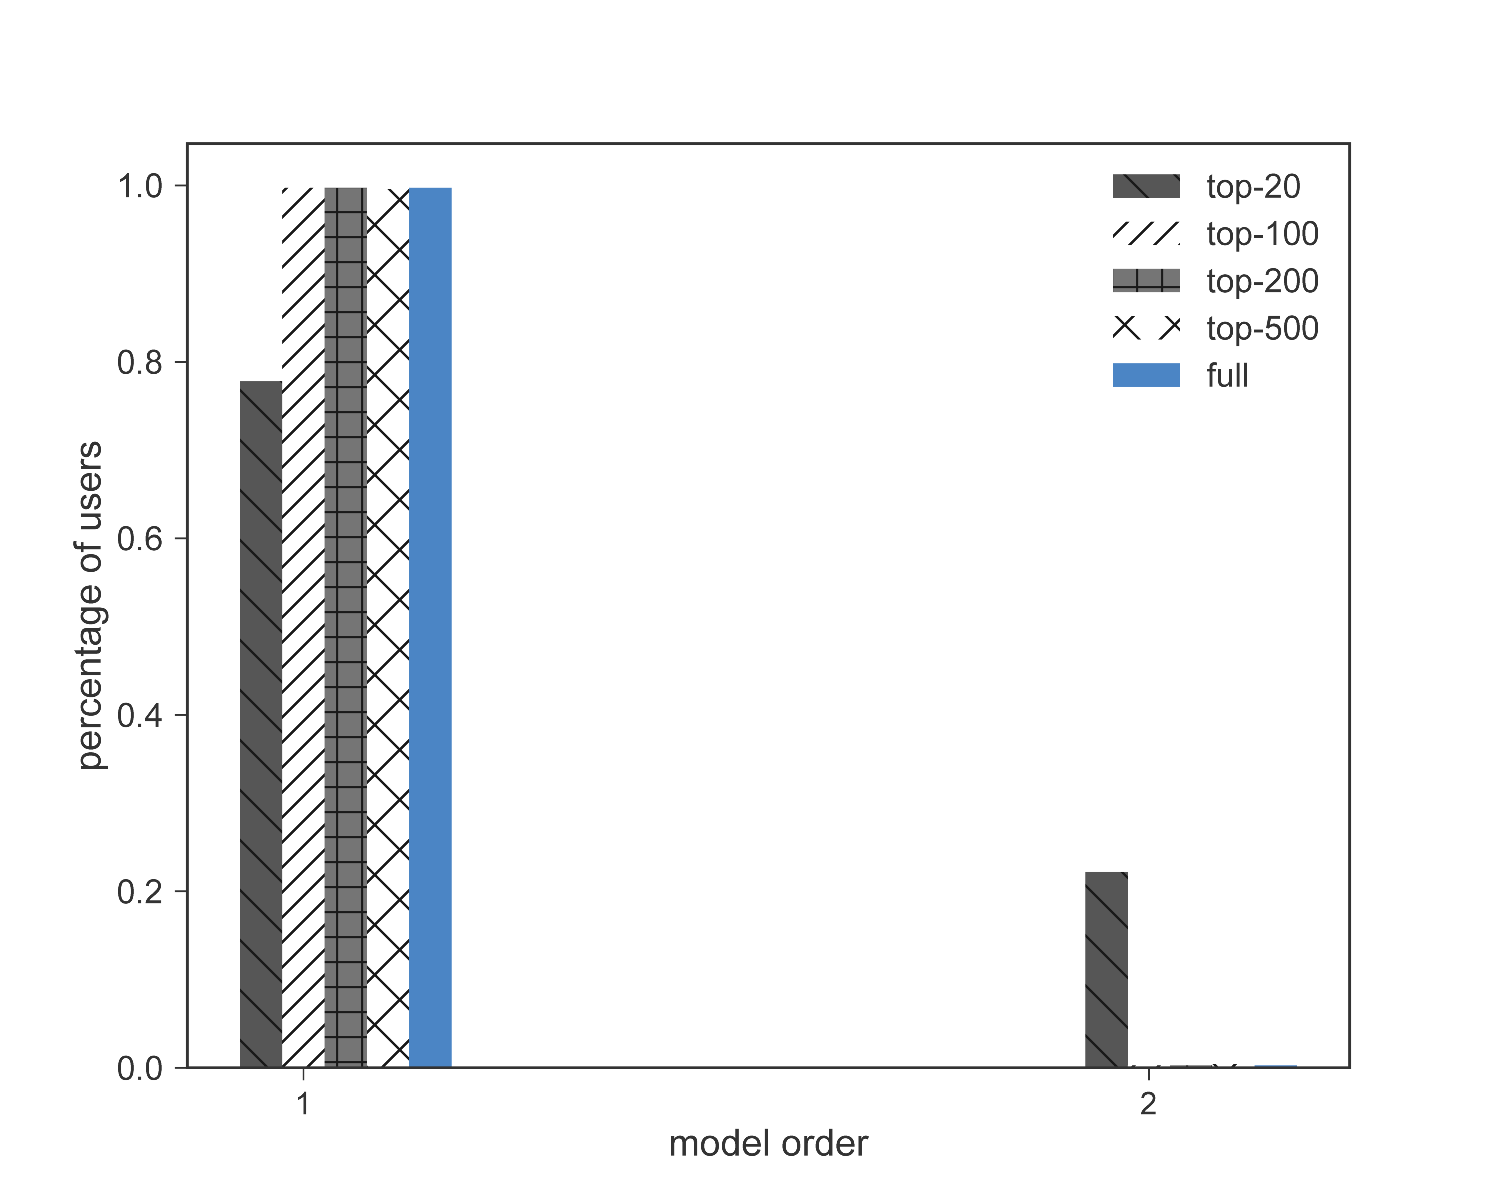
\includegraphics[totalheight=8cm]{\MyPath/fig/model_selection_.pdf}
	\caption{{Optimal order for increasing number of locations.}}
	\label{fig:model_selection}
\end{figure*}

We began by selecting the optimal order of the network representations derived from the mobility trajectories of the $1,500$ handsets selected from the Device Analyzer dataset.
We first parsed the \emph{cid} sequences from the mobility trajectories into mobility networks.
In order to remove \emph{cid}s associated with movement, we only defined nodes for \emph{cid}s which were visited by the handset for at least 15 minutes.
Movements from one \emph{cid} to another were then recorded as edges in the mobility network.

As outlined in~\cref{sec:graph-k-anonymity}, we analysed the pathways of the Device Analyzer dataset during the entire observation period, applying the model selection method~\cite{scholtes2017network} of Scholtes.\footnote{\url{https://github.com/IngoScholtes/pathpy}}
This method tests graphical models of varying orders and selects the optimal order by balancing the model complexity and the explanatory power of observations.

We tested higher-order models up to order three. In the case of top$-20$ mobility networks, we found routine patterns in the mobility trajectories were best explained with models of order two for more than 20$\%$ of the users. However, when considering top$-100$, top$-200$, top$-500$ and full mobility networks, we found that the optimal model for our dataset has order one for more than $ 99\% $ of the users; see~\cref{fig:model_selection}. In other words, when considering mobility trajectories which visit less frequent locations in the graph, the overall increase in likelihood of the data for higher-order models cannot compensate for the complexity penalty induced by the larger state space. So while there might still be regions in the graph which are best represented by a higher-order model, the optimal order describing the entire graph is one. Therefore we use a model of order one in the rest of this paper.

\subsection{Data properties and statistics} \label{sec:data-stats}

\begin{table*}[!t]
	\centering 
		\resizebox*{\textwidth}{!}{
			\begin{tabular}{| c | c | c | c | c | c | c | c | c |}
				\hline
				\textbf{Networks} & \vtop{\hbox{\strut \;\;\;\textbf{\# of}}\hbox{\strut \textbf{networks}}}  &  \vtop{\hbox{\strut \textbf{Num. of}}\hbox{\strut \textbf{nodes,~avg.}}}  &  \vtop{\hbox{\strut \textbf{Edges,}}\hbox{\strut \;\;\;\textbf{avg.}}} & \vtop{\hbox{\strut \textbf{Density,}}\hbox{\strut \;\;\;\textbf{avg.}}} & \vtop{\hbox{\strut \;\;\;\;\;\;\textbf{Avg.}}\hbox{\strut \textbf{clust. coef.}}} & \vtop{\hbox{\strut \textbf{Diameter,}}\hbox{\strut \;\;\;\;\;\;\textbf{avg.}}}  & \vtop{\hbox{\strut \;\;\;\;\;\textbf{Avg.}}\hbox{\strut \textbf{short.~path}}} & \vtop{\hbox{\strut \textbf{Recurrence}}\hbox{\strut \;\;\;\;\;\textbf{rate~($\%$)}}}   \\
				\hline
				\text{top$-50$ locations}& $1,500$ & $49.9\pm1.3$  & $236.6\pm78.1$ & $0.19\pm0.06$ & $0.70\pm0.07$ & $3.42\pm0.86$  & $1.93\pm0.20$ & $84.7\pm5.6$\\
				\hline
				\text{top$-100$ locations}& $1,500$ & $98.3\pm7.9$   & $387.1\pm144.7$ & $0.08\pm0.03$ & $0.60\pm0.10$ & $4.67\pm1.48$  & $2.33\pm0.40$& $78.3\pm7.8$\\
				\hline
				\text{top$-200$ locations}& $1,500$ & $179.2\pm37.8$ & $548.2\pm246.1$ & $0.04\pm0.02$ & $0.47\pm0.12$ & $7.52\pm4.21$  & $3.07\pm1.18$ &$73.0\pm9.9$\\
				\hline
				\text{full } & $1,500$ & $334.6\pm235.8$  & $741.6\pm527.3$ & $0.02\pm0.02$ & $0.33\pm0.09$ & $15.98\pm10.18$  & $4.84\pm2.93$ & $68.8\pm12.3$\\
				\hline
			\end{tabular}	
		}\caption{Summary statistics of mobility networks in the Device Analyzer dataset.}
		\label{tab:summary-statistics}
\end{table*}	

\begin{figure*}[!t]
	\centering
	\begin{subfigure}[!t]{0.47\textwidth}
		\centering		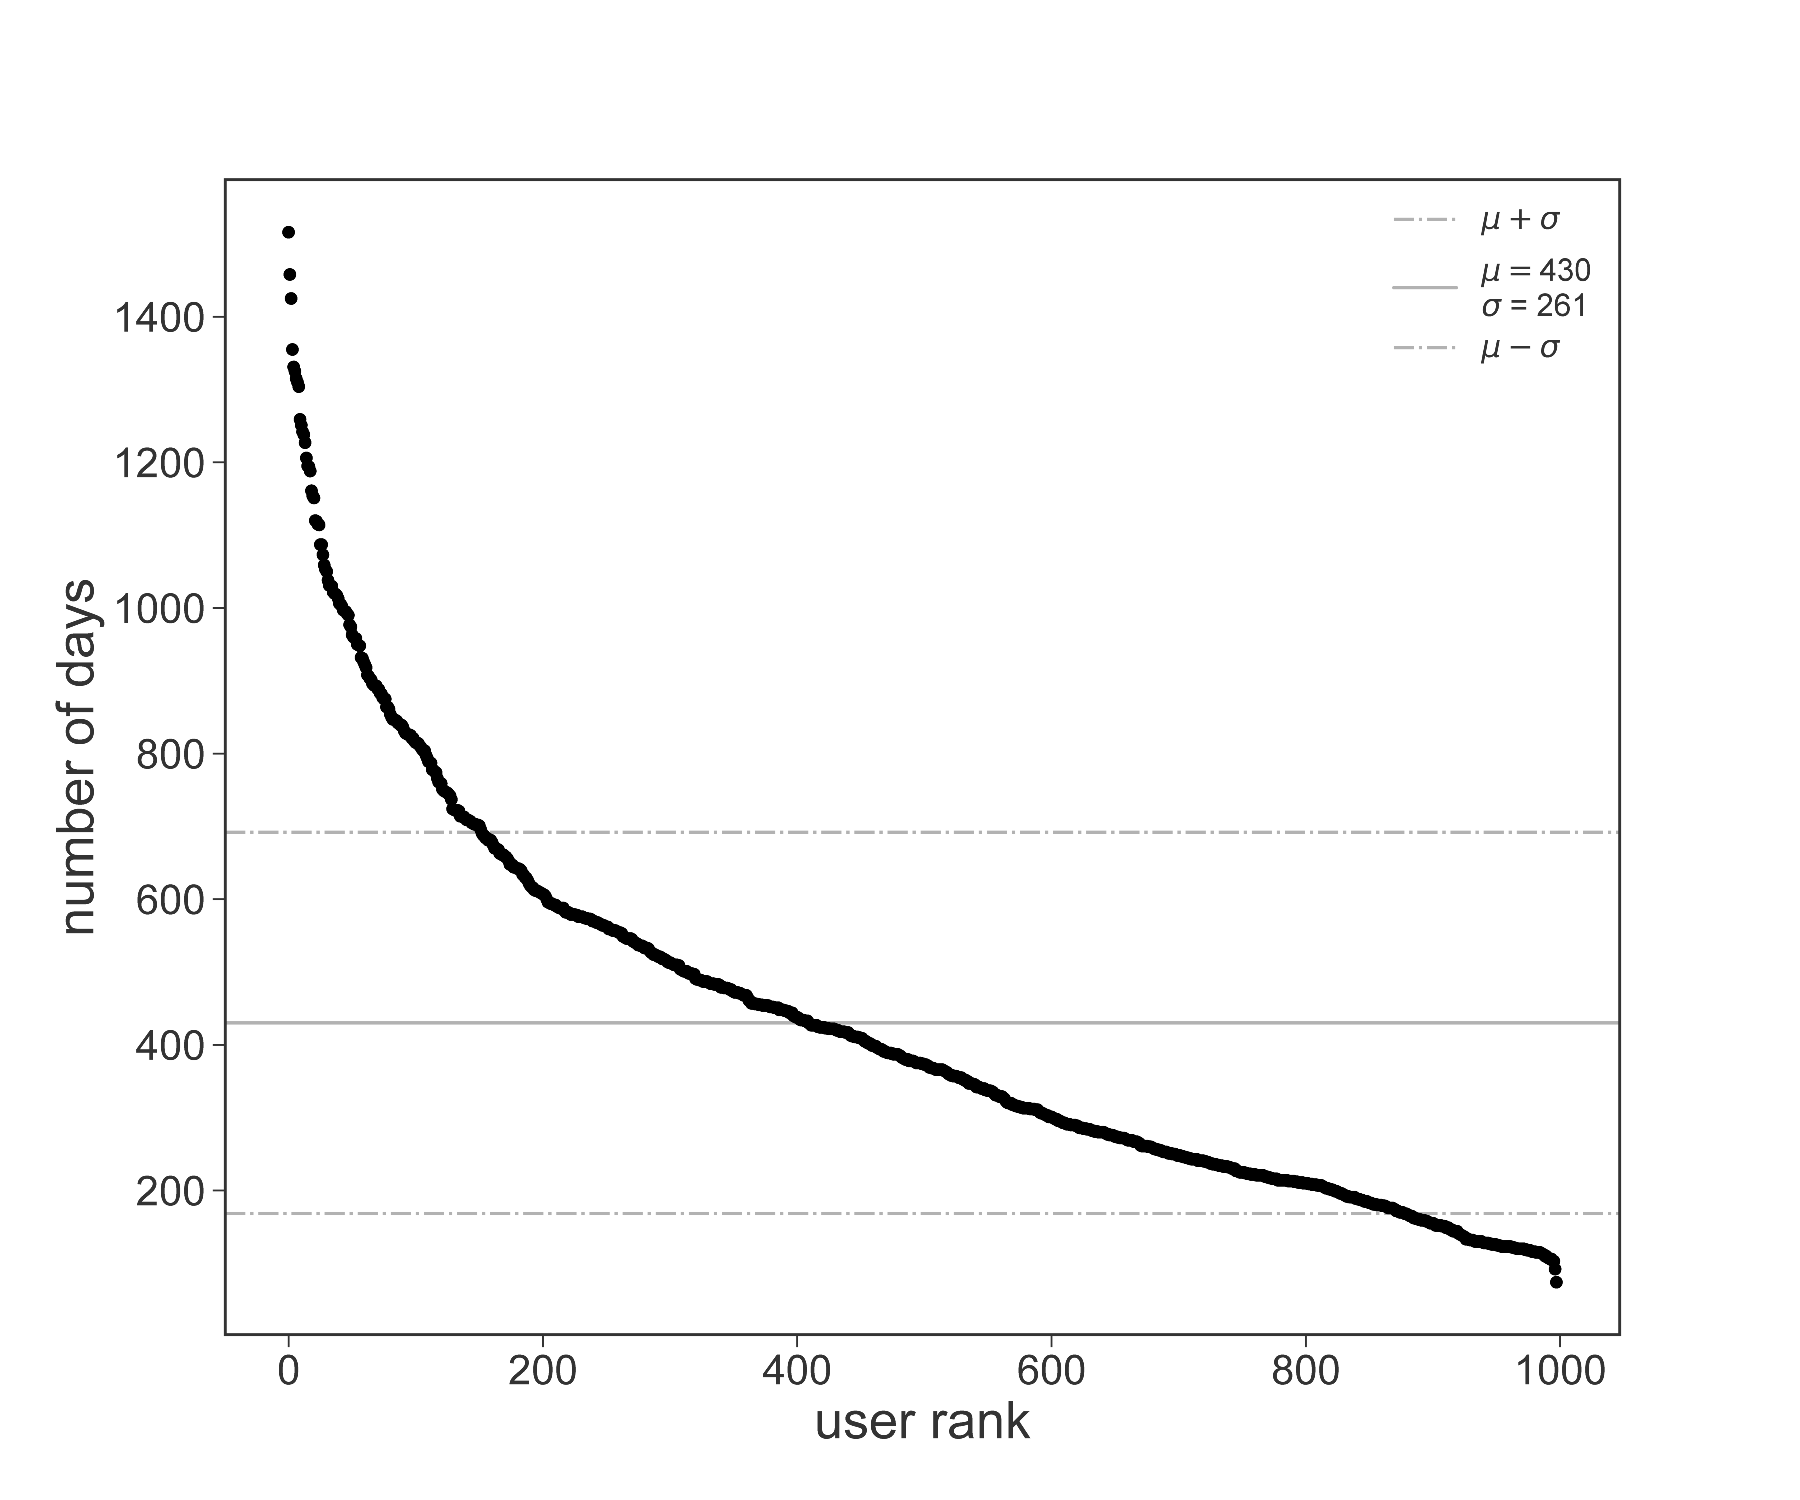
\includegraphics[width=0.9\textwidth]{\MyPath/fig/observation_window_.pdf}
		\caption{}
		\label{fig:num_of_days}
	\end{subfigure}%
	\begin{subfigure}[!t]{.47\textwidth}
		\centering
		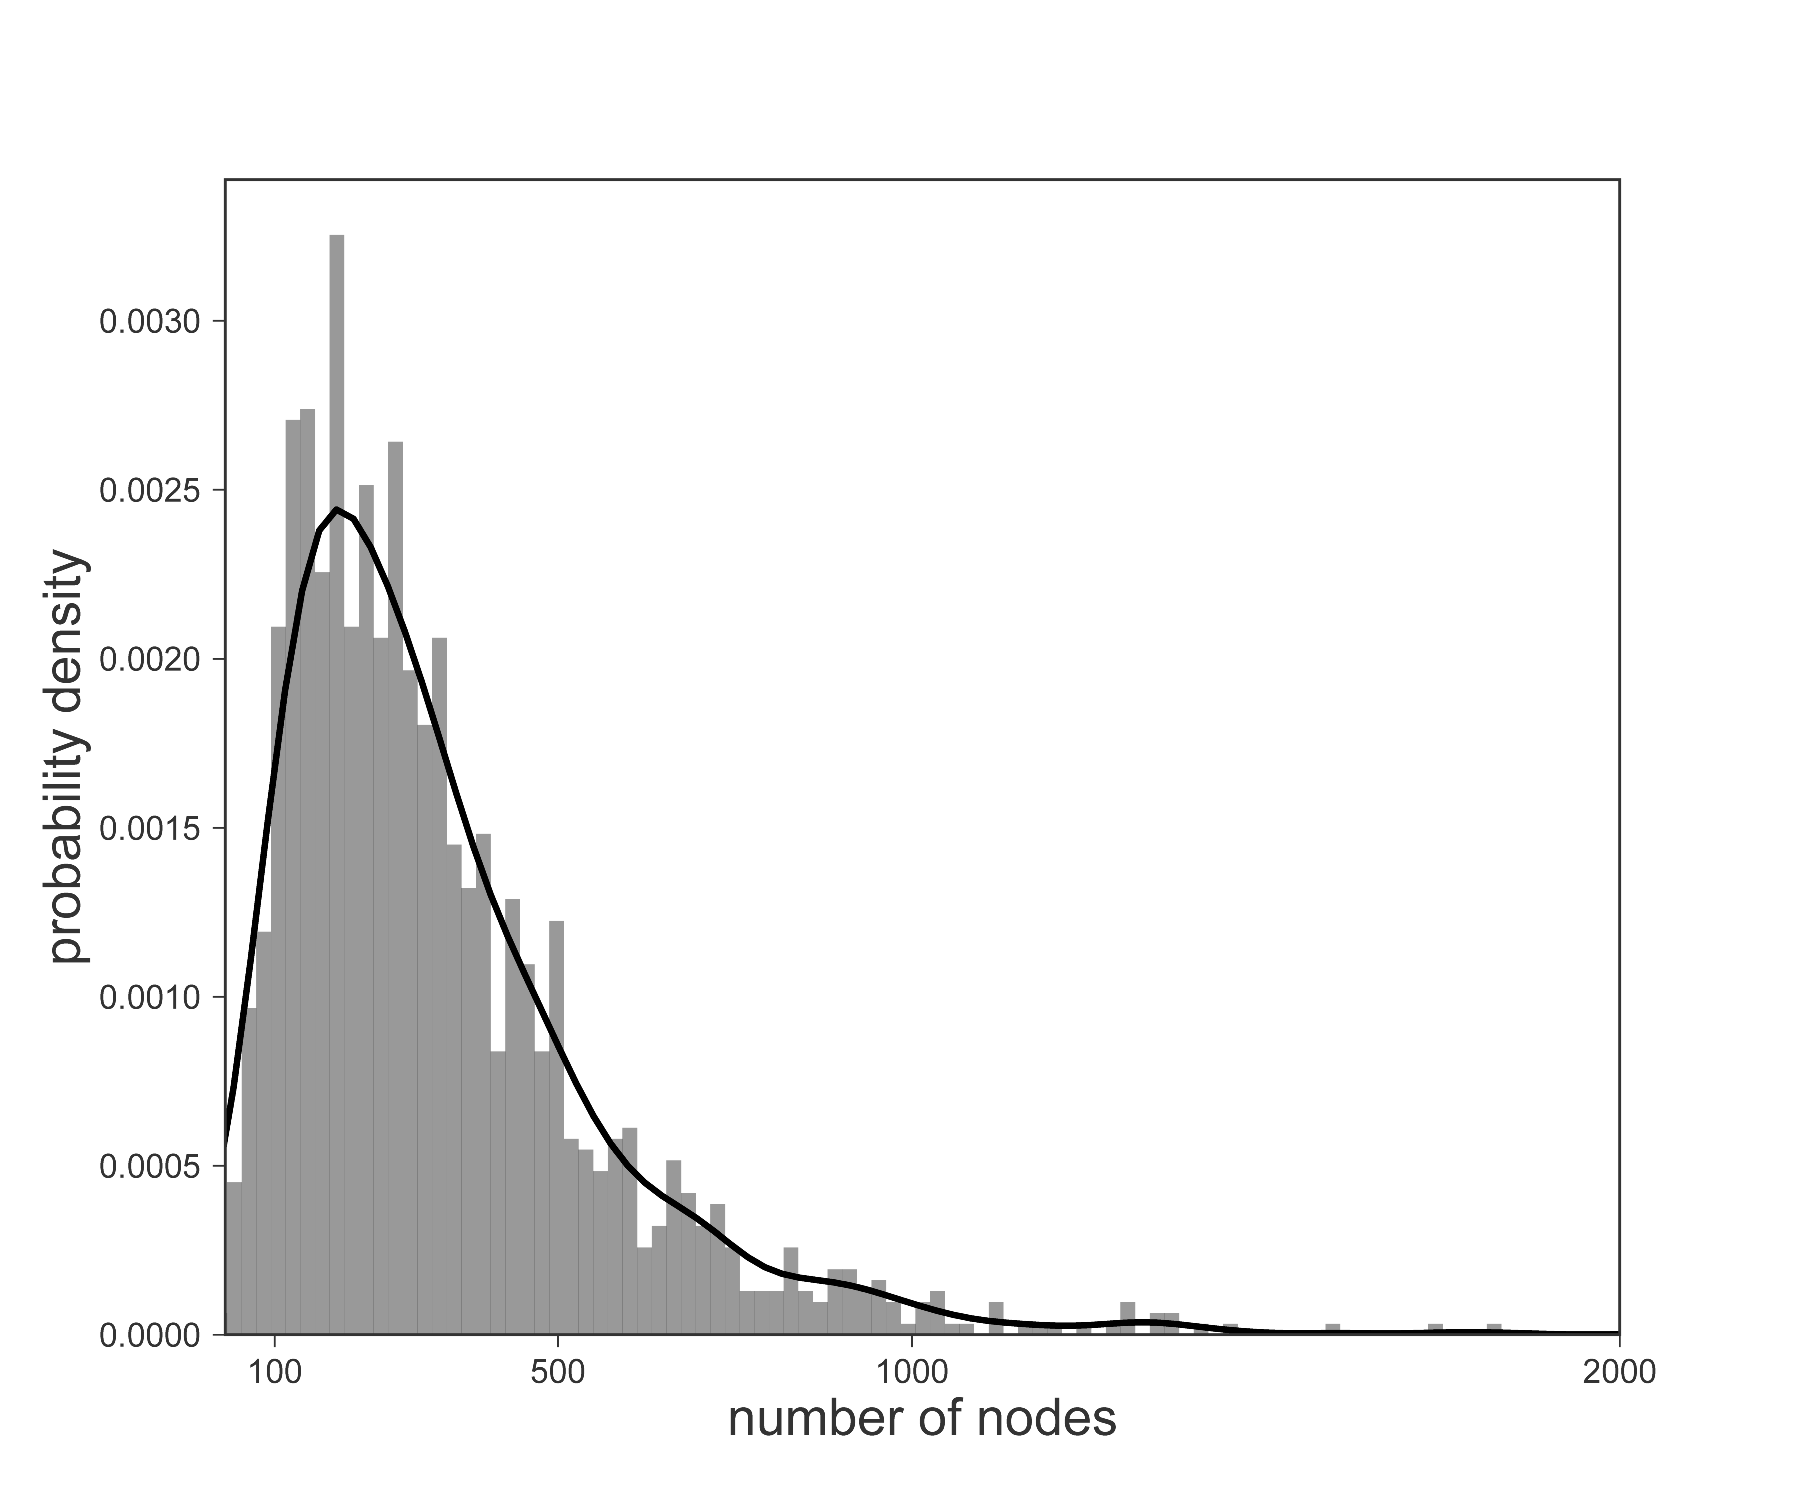
\includegraphics[width=0.9\textwidth]{\MyPath/fig/unnorm_full_graphspdf_netsize_.pdf}
		\caption{}
		\label{fig:sizes}
	\end{subfigure}%
	\\
	\begin{subfigure}[!t]{0.47\textwidth}
		\centering
		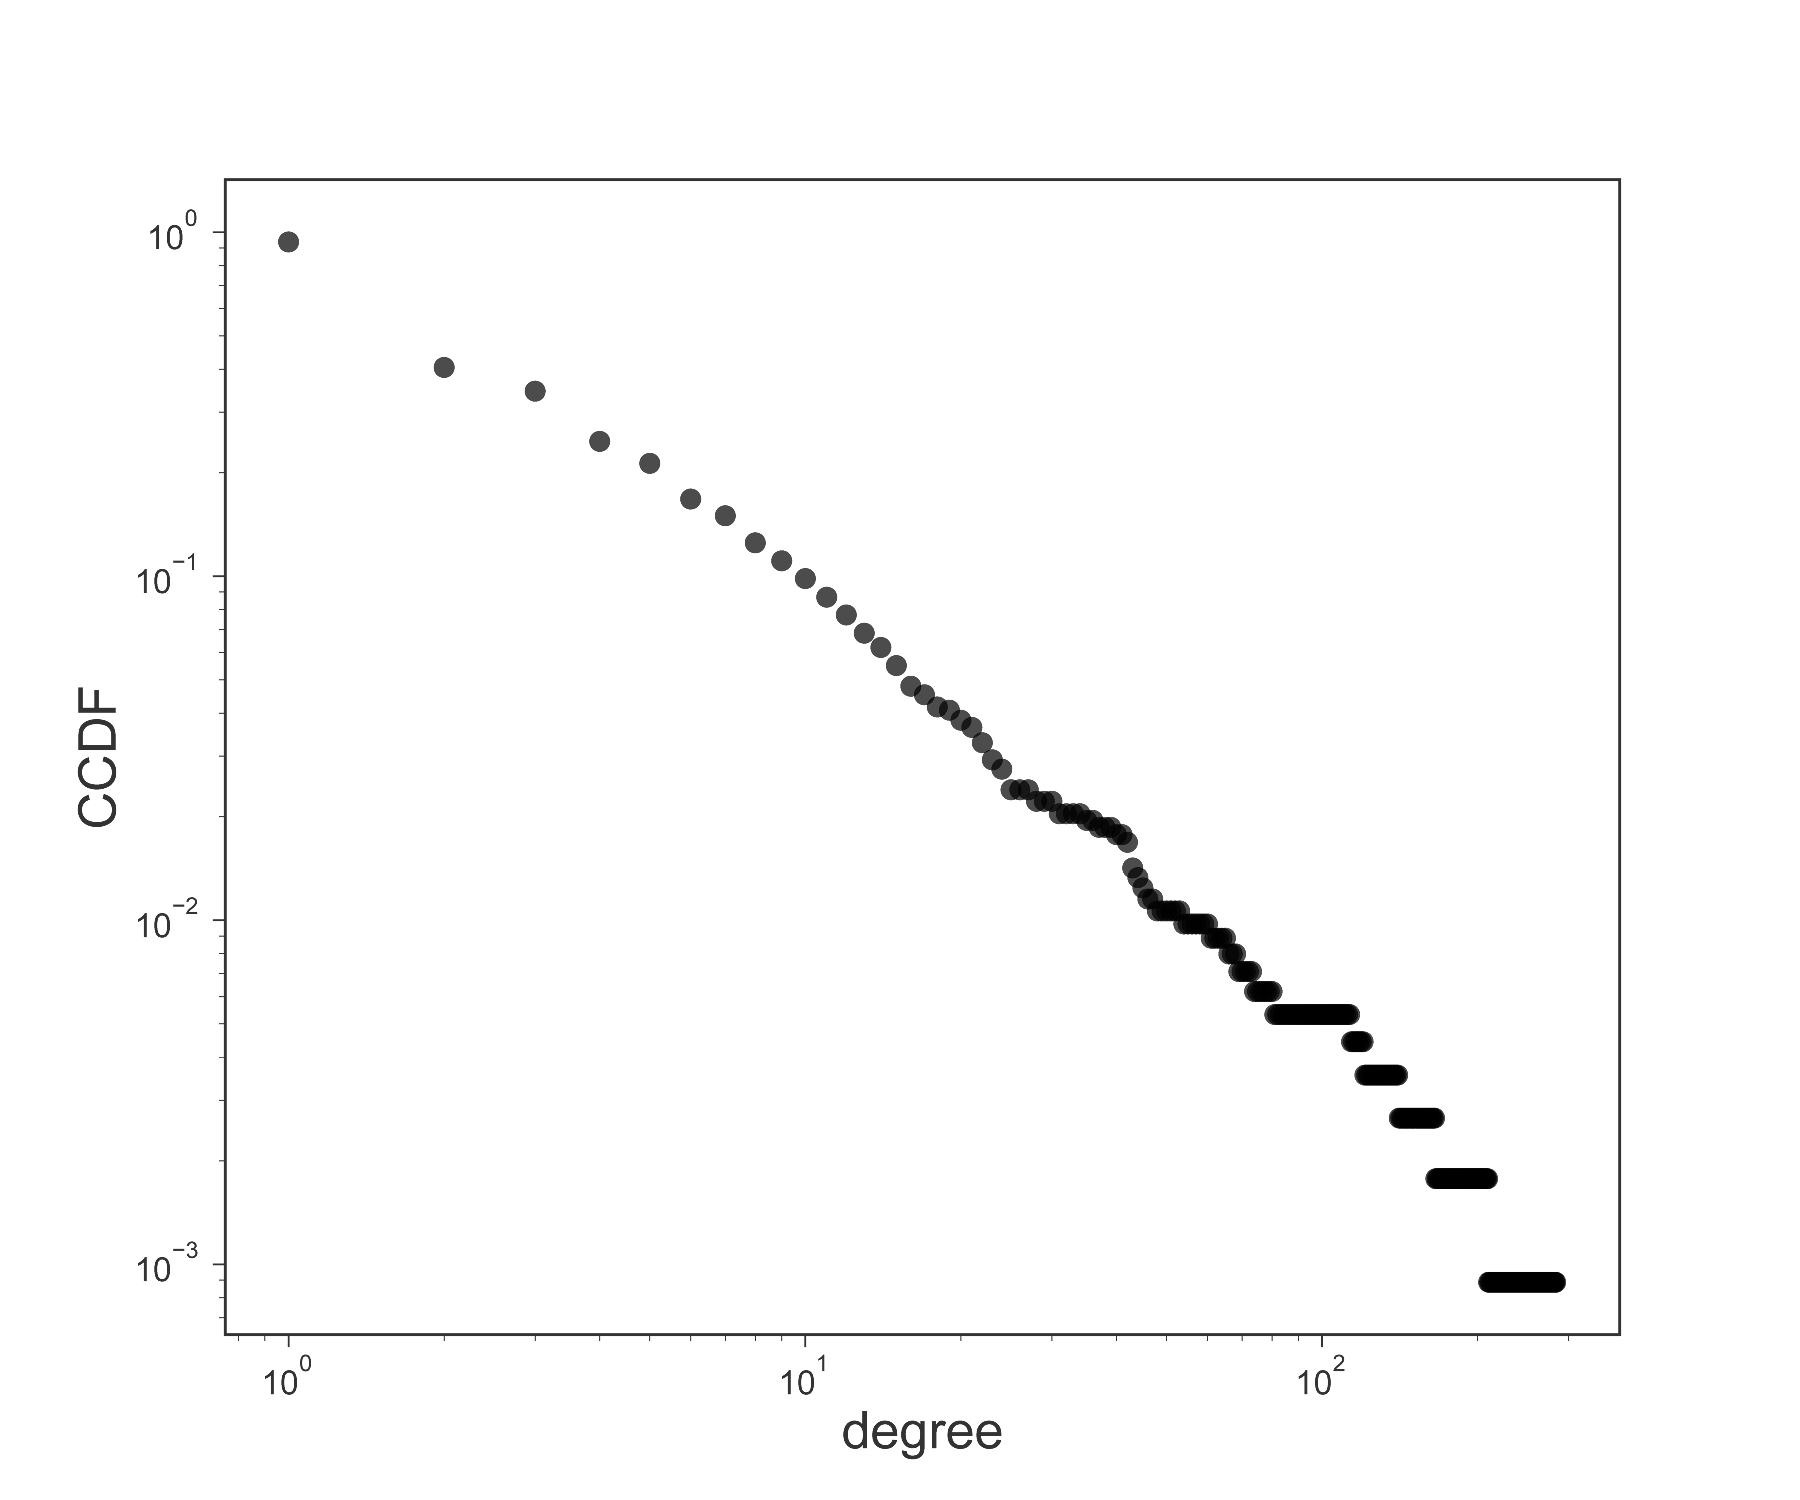
\includegraphics[width=0.9\textwidth]{\MyPath/fig/183_degree_ccdf_.pdf}
		\caption{}
		\label{fig:ccdf}
	\end{subfigure}
	\begin{subfigure}[!t]{0.47\textwidth}
		\centering
		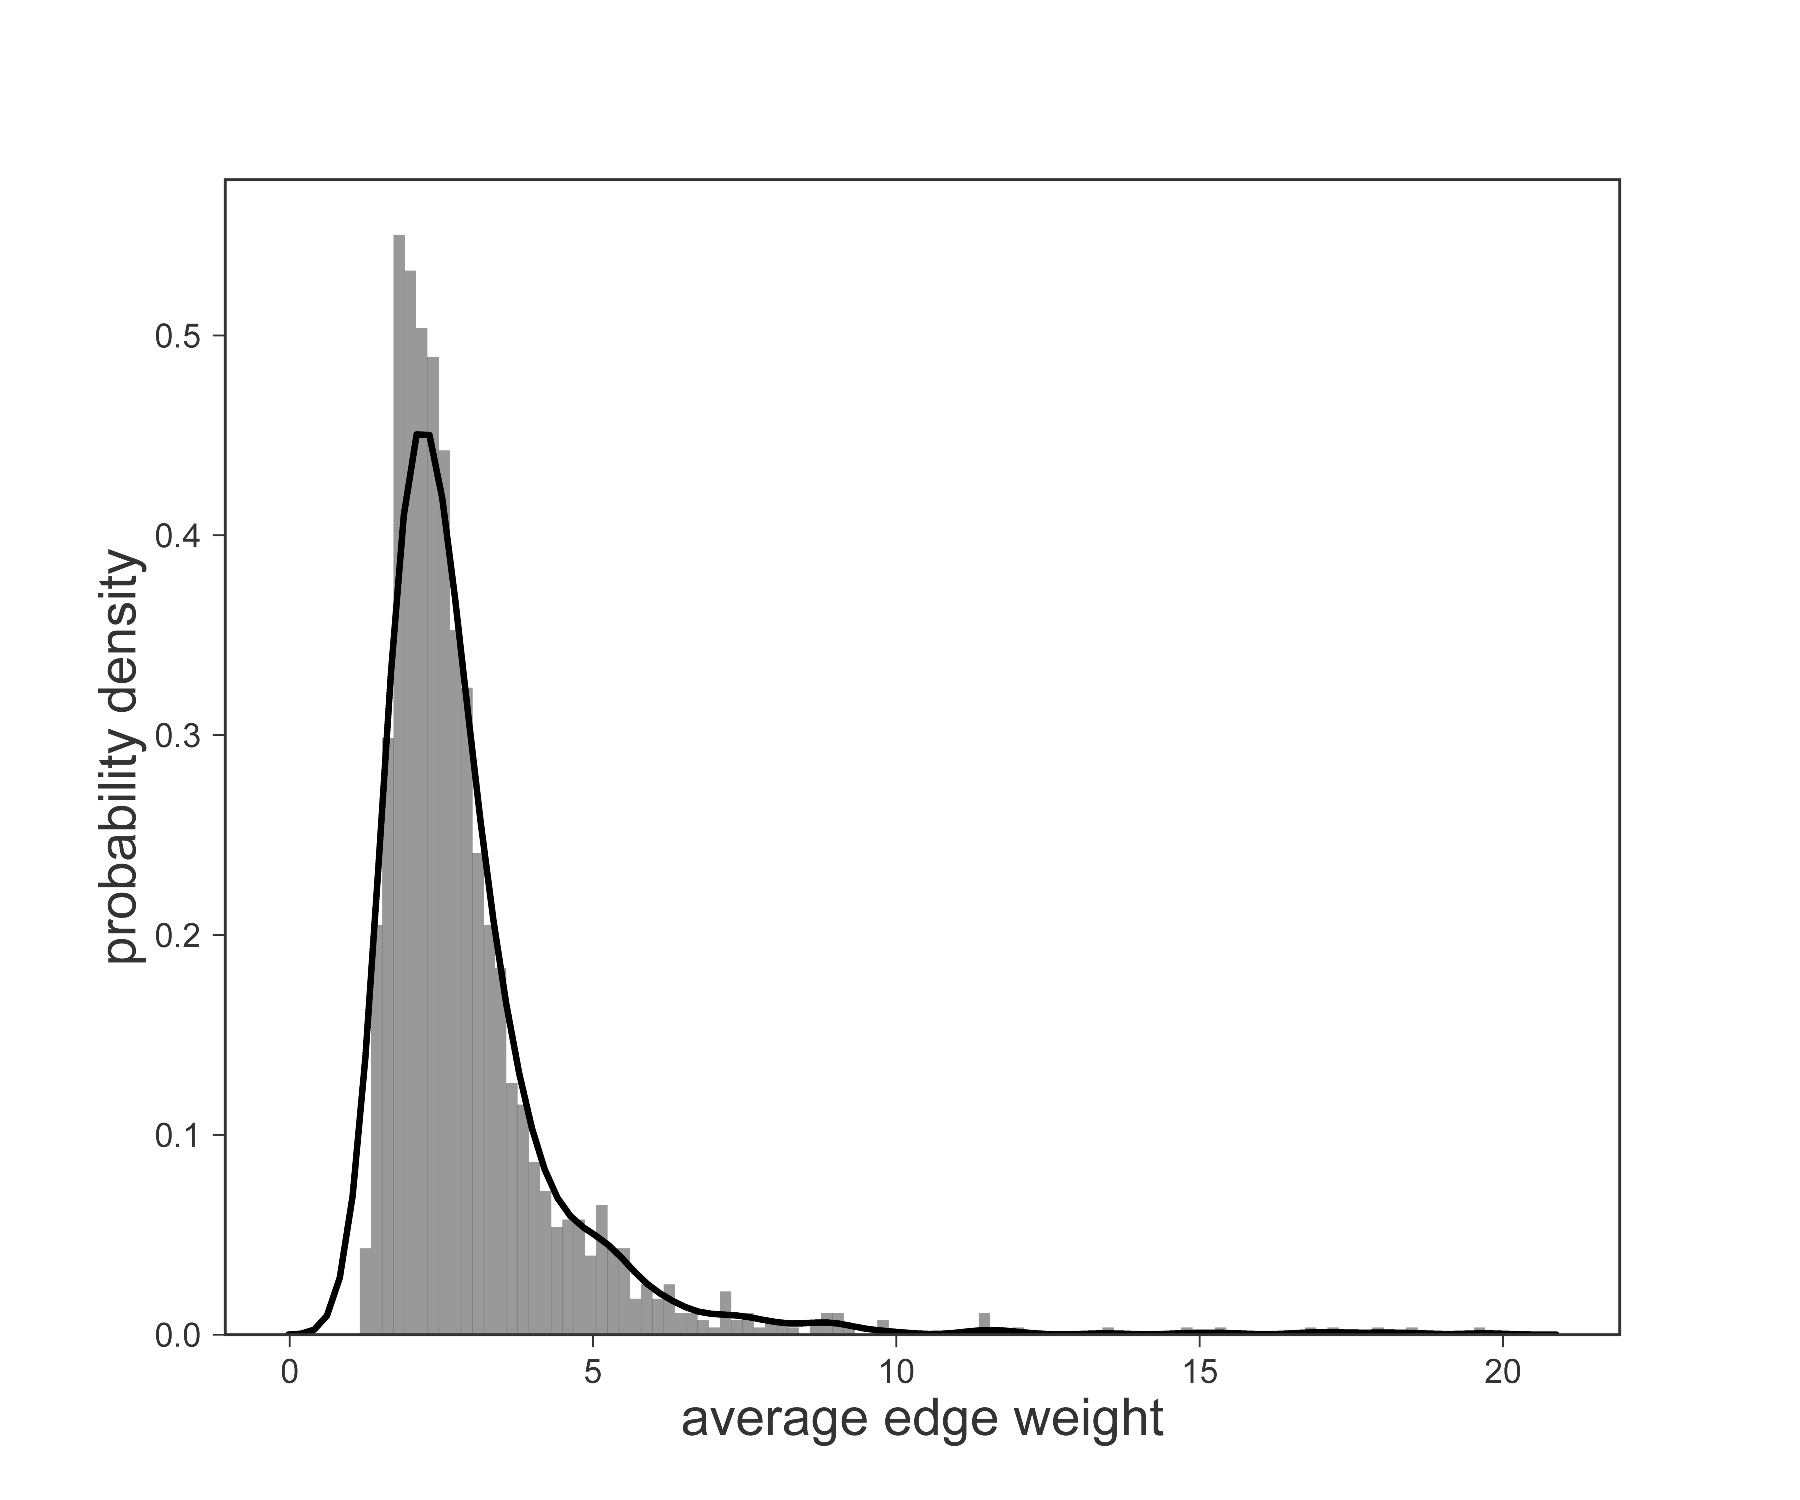
\includegraphics[width=0.9\textwidth]{\MyPath/fig/unnorm_full_graphspdf_avg_edge_weight_.pdf}
		\caption{}
		\label{fig:avg_edge_weight}
	\end{subfigure}
	\caption{Empirical statistical findings of the Device Analyzer dataset. (a)~Observation period duration distribution. (b)~Normalized histogram and probability density estimate of network size for the full mobility networks over the population. (c)~Complementary cumulative distribution function (\emph{CCDF}) for the node degree in the mobility network of a typical user from the population, displayed on log-log scale. (d)~Normalized histogram and probabilty density of average edge weight over the networks.}
	\label{fig:eda}
\end{figure*}

In~\cref{tab:summary-statistics} we provide a statistical summary of the original and the pruned versions of the mobility networks. We observe that allowing more locations in the network implies an increase in the variance of their statistics, and leads to smaller density, larger diameter and larger average shortest-path values.

A \emph{recurrent edge traversal} in a mobility network occurs when a previously traversed edge is traversed for a second or subsequent time.
We then define \emph{recurrence rate} as the percentage of edge traversals which are recurrent.
We find that mobility networks display a high recurrence rate, varying from  $68.8\%$ on average for full networks to $84.7\% $ for the top$-50$ networks, indicating that the mobility of the users is mostly comprised of repetitive transitions between a small set of nodes in a mobility network.

\cref{fig:sizes} displays the normalized histogram and probability density estimate of network size for full mobility networks.
We observe that sizes of few hundred nodes are most likely in our dataset, however mobility networks of more than $1,000$ nodes also exist.
Reducing the variance in network size will be proved helpful in cross-network similarity metrics, hence we also consider truncated versions of the networks.

As shown in~\cref{fig:ccdf}, the parsed mobility network of a typical user is characterized by a \emph{heavy-tailed degree distribution}. We observe that a small number of locations have high degree and correspond to dominant states for a person's mobility routine, while a large number of locations are only visited a few times throughout the entire observation period and have a small degree.

 \cref{fig:avg_edge_weight} shows that the estimated probability distribution of average edge weight.
 This peaks in the range from two to four, indicating that many transitions captured in the full mobility network are rarely repeated. However, most of the total weight of the network is attributed to the tail of this distribution, which corresponds to the edges that the user frequently repeats.

\subsection{Anonymity clusters on top$-N$  networks}\label{sec:anonymity-clusters}

\begin{table*}[!t]
	\centering
		\resizebox*{0.7\textwidth}{!}{
			\begin{tabular}{|c|c|c|c|c|c|c|}
				\hline
				\textbf{N}             & 4    & 5           & 6           & 7            & 8             & 9         \\ \hline
				\textbf{\# undirected} & 11   & 34          & 156         & 1,044         & 12,346         & 274,668    \\ \hline
				\textbf{N}             & 4    & \multicolumn{2}{c|}{5}    & \multicolumn{2}{c|}{6}       & 7         \\ \hline
				\textbf{\# directed}   & 2,128 & \multicolumn{2}{c|}{9,608} & \multicolumn{2}{c|}{1,540,944} & 882,033,440 \\ \hline
			\end{tabular}
		}\caption{Sequences of non-isomorphic graphs for undirected and directed graphs of increasing size.}
	\label{tab:graphsenumeration}
\end{table*}

We examine to what extent the heterogeneity of users mobility behaviour can be expressed in the topology of the state connectivity networks.
For this purpose, we generate the isomorphism classes of the top$-N$ networks of our dataset for increasing network size $ N $.
We then compute the graph $k-$anonymity of the population and the corresponding identifiability set.
This analysis demonstrates empirically the privacy implications of releasing anonymized users pathway information at increasing levels of granularity.

Before presenting our findings on the Device Analyzer dataset, we will perform a theoretical upper bound analysis on the identifiability of a population, by finding the maximum number of people that can be distinguished by networks of size $ N $.
This corresponds to the number of non-isomorphic graphs with $ N $ nodes.

Currently the most of efficient way of enumerating  non-isomorphic graphs is by using McKay's algorithm~\cite{McKay}, implemented in the package~\texttt{nauty}.\footnote{\url{http://pallini.di.uniroma1.it/}}~\cref{tab:graphsenumeration} presents the enumeration for undirected and directed non-isomorphic graphs of increasing size. We observe that there exist $12,346$ undirected graphs with $8$ nodes and $9,608$ directed graphs with $5$ nodes. In other words, finding the top$-8$ places for each person is the smallest number which could produce unique graphs for each person in our sample of $1,500$ individuals; this reduces to $5$ when directionality is taken into account. Moreover, we find that top$-12$ undirected and top$-8$ directed networks are sufficient to enable each human on the planet to be represented by a different graph, assuming world population of $7.6$B.

Next we present the results of our analysis on the Device Analyzer data.
As observed in~\cref{fig:k_an}, \emph{sparsity arises in a mobility network even for very small $ N $}.
In particular, in the space of undirected \emph{top$-4$} location networks, there is already a cluster with only $ 3 $ members, while for all $ N > 4 $ there always exist isolated isomorphic clusters.
\emph{$ k-$anonymity} decreases to $ 1 $ even for $ N=3 $ when considering directionality.
Moreover, the \emph{identifiability set} dramatically increases with the size of network: approximately $ 60\% $ of the users are uniquely identifiable from their top$-10$ location network.
This percentage increases to $93\%$ in directed networks.
For the entire population of the $ 1,500 $ users, we find that 15 and 19 locations suffice to form uniquely identifiable directed and undirected networks respectively.

The difference between our empirical findings and our theoretical analysis suggests that large parts of the top$-N$ networks are common to many people.
This can be attributed to patterns that are widely shared (e.g.\ the trip from work to home, and from home to work).

\begin{figure*}[!t]
	\begin{subfigure}[t]{0.49\textwidth}
		\centering
		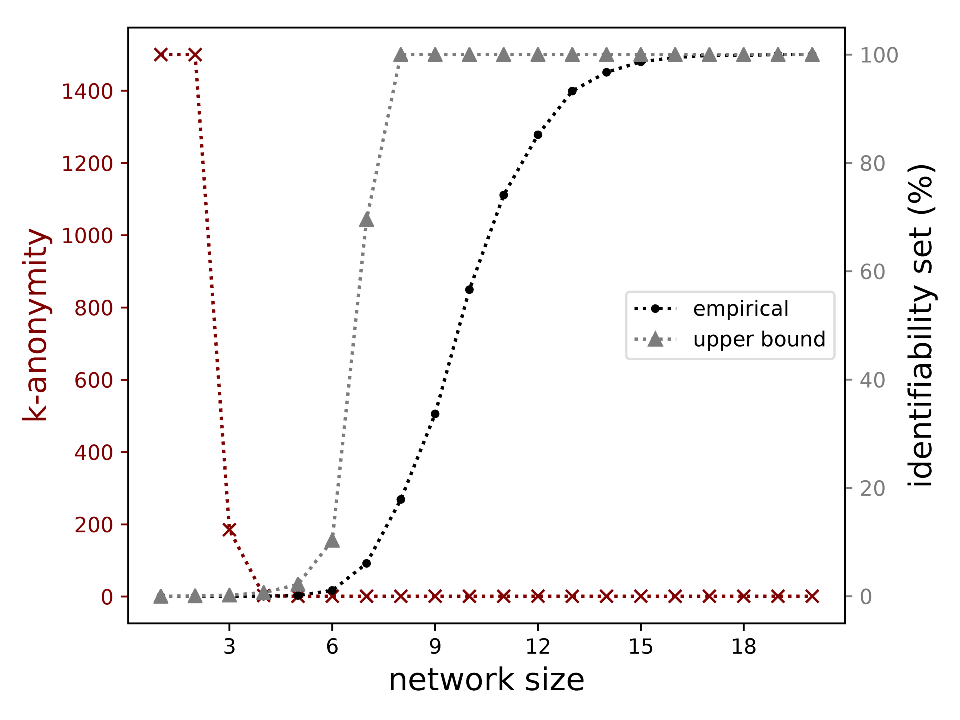
\includegraphics[height=5.5cm]{\MyPath/fig/k_anonymity_undirected_.pdf}
		\caption{\centering {Undirected top$-N$ networks.}}
		\label{fig:k_an_un}
	\end{subfigure}%
	\begin{subfigure}[t]{0.49\textwidth}
		\centering
		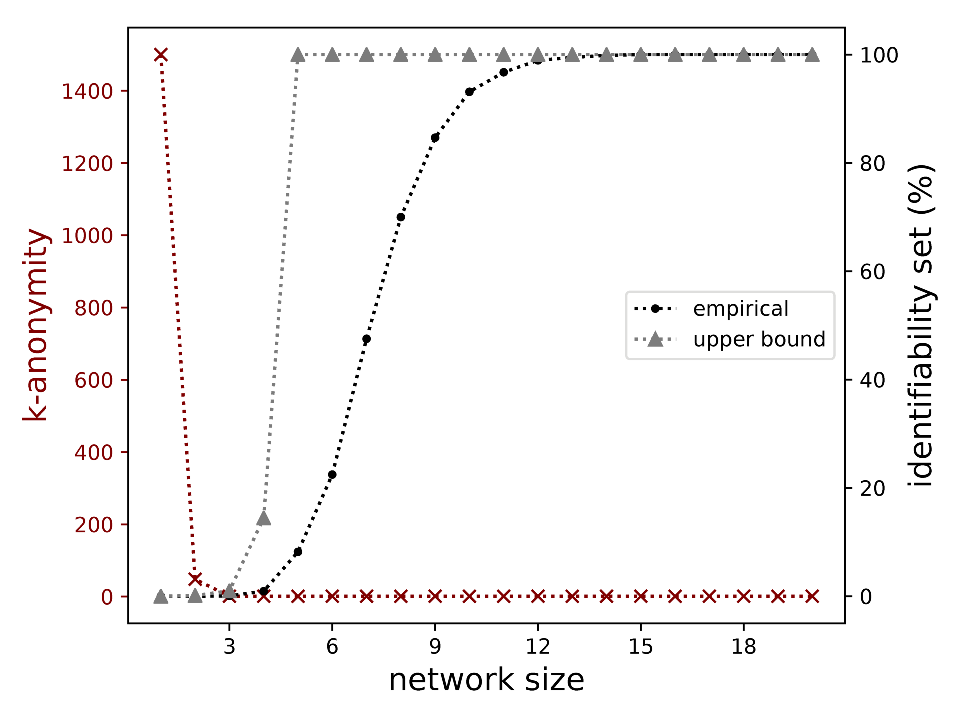
\includegraphics[height=5.5cm]{\MyPath/fig/k_anonymity_dir_.pdf}
		\caption{\centering {Directed top$-N$ networks.}}
		\label{fig:k_an_dir}
	\end{subfigure}%
	\caption{{Identifiability set and $k-$anonymity for undirected and directed top$-N$ mobility networks for increasing number of nodes. Displayed is also the theoretical upper bound of identifiability for networks with $ N $ nodes.}
	}
	\label{fig:k_an}
\end{figure*}

\begin{figure*}[!t]
	\begin{subfigure}[t]{0.49\textwidth}
		\centering
		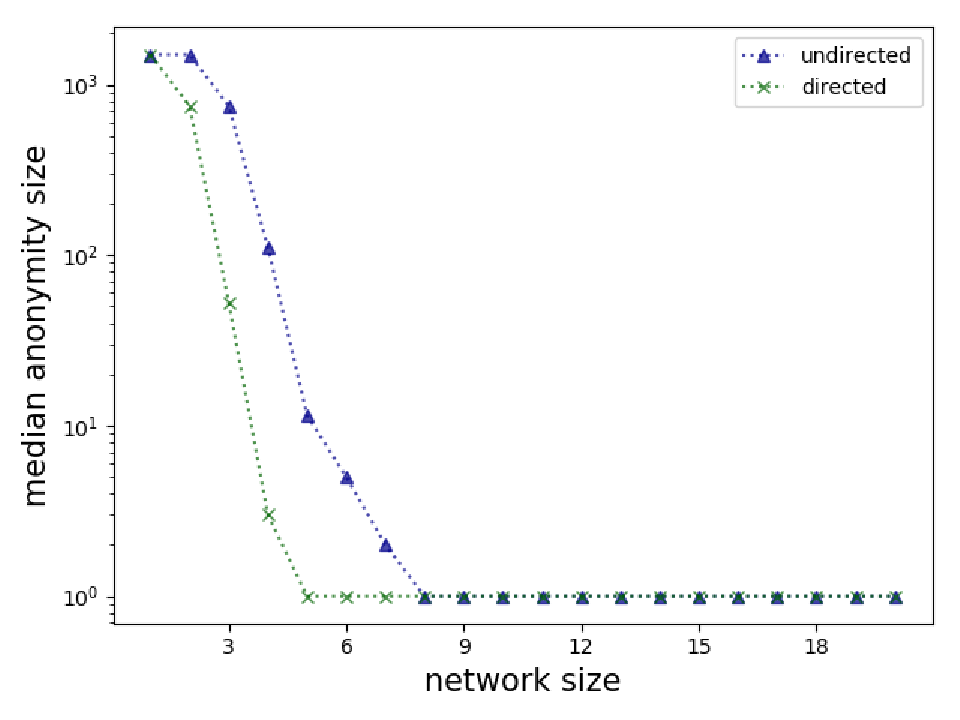
\includegraphics[height=5cm]{\MyPath/fig/median_k_anonymity_.pdf}
		\caption{\centering {Median anonymity size.}}
		\label{fig:k_an_med}
	\end{subfigure}
	\begin{subfigure}[t]{0.49\textwidth}
		\centering
		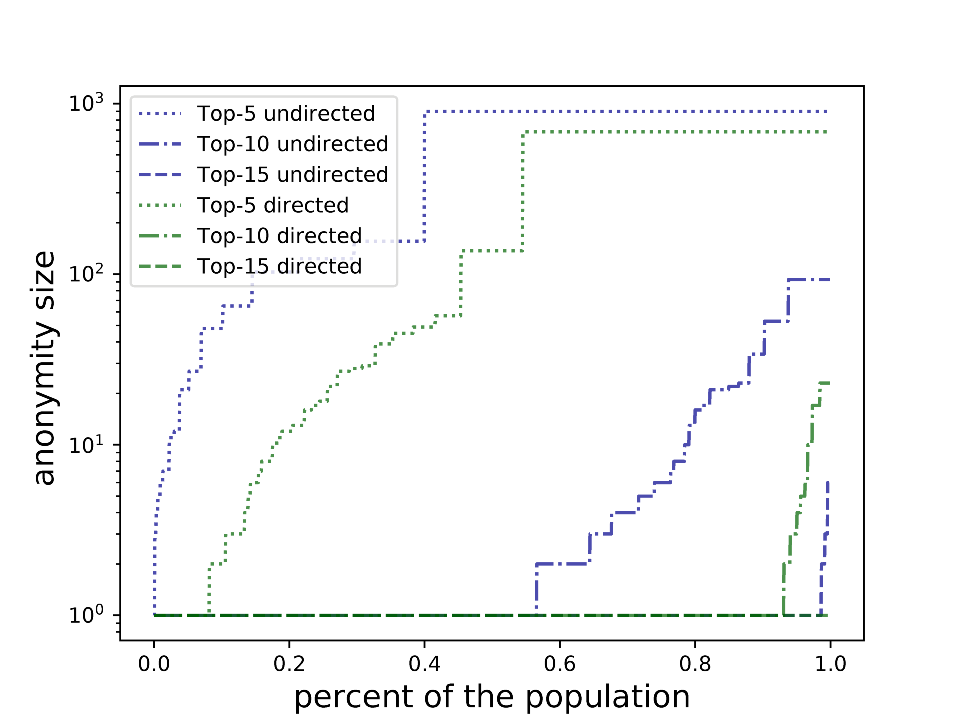
\includegraphics[height=5.5cm]{\MyPath/fig/anonymity_distribution_.pdf}
		\caption{\centering {Cumulative distribution of the anonymity size.}}
		\label{fig:anon_distribution}
	\end{subfigure}
	\caption{{Anonymity size statistics over the population of top$-N$ mobility networks for increasing network size.}}
	\label{fig:k_an_stats}
\end{figure*}

 \cref{fig:k_an_stats} shows some additional statistics of the anonymous isomorphic clusters formed for varying network sizes.
 Median anonymity becomes one for network sizes of five and eight in directed and undirected networks respectively; see~\cref{fig:k_an_med}.
 In~\cref{fig:anon_distribution} we observe that the population arranges into clusters with small anonymity even for very small network sizes: around $5\%$  of the users have at most $10$-anonymity when considering only five locations in their network, while this percentage increases to $80\%$ and $100\% $ for networks with $10$ and $15$ locations.
 This result confirms that anonymity is even harder when the directionality of edges are provided, since the space of directed networks is much larger than the space of the undirected networks with the same number of nodes.

 The above empirical results indicate that the diversity of individuals mobility is reflected in the network representations we use, thus we can meaningfully proceed to discriminative tasks on the population of mobility networks.